\section{Structured Query Language (SQL)}
\begin{itemize}
    \item SQL is a language used for interacting with relational Database Management Systems (RDBMS)
    \item It is kind of like a programming language, it is not strictly a programming language.
    \item You can use SQL to get the RDBMS to do things for you.
        \begin{itemize}
            \item Create, Retrieve, Update and Delete data.
            \item Create and Manage database.
            \item Design and create database tables.
            \item Perform administration tasks (security, user management, import/export, etc)
        \end{itemize}
    
    \item RDBMS do not speak English, they speak SQL.
    \item SQL implementations vary between systems:
        \begin{itemize}
            \item Not all RDBMS' follow the SQL standard to a 'T'.
            \item The concepts are the same but the implementation may vary.
            \item Keep in mind that certain instructions might work on certain RDBMS and not work on others.
        \end{itemize}
    
    \item SQL is actually a hybrid language, it's basically 4 types of languages in one:
        \begin{itemize}
            \item It is a Data Query Language (DQL):
                \begin{itemize}
                    \item Used to query the database for information.
                    \item Get information that is already stored there.
                \end{itemize}
            
            \item Data Definition Language (DDL):
                \begin{itemize}
                    \item Used for defining database schema (A schema is the overall layout of the database such as what columns and rows it will have, what data types are they going to be able to store.)
                \end{itemize}
            
            \item Data Control Language (DCL):
                \begin{itemize}
                    \item Used for controlling access to the data in the database.
                    \item Users and permissions management.
                \end{itemize}
            
            \item Data Manipulation Language (DML):
                \begin{itemize}
                    \item Used for inserting, updating and deleting data from the database.
                \end{itemize}
        \end{itemize}
\end{itemize}

\section{Queries}
\begin{itemize}
    \item A query is a set of instructions given to the RDBMS (written in SQL) that tell the RDBMS what information you want it to retrieve for you.
        \begin{itemize}
            \item There are TONS of data in a database.
            \item Often hidden in a complex schema.
            \item The goal is to only get the data you need.
        \end{itemize}
    
    \item Example: if we want to query the ages and the names of employees in a company that make more than 30000.
        \begin{minted}[autogobble]{sql}
            SELECT employee.first_name, employee.last_name 
            FROM employee 
            WHERE employee.salary >30000;
        \end{minted}
        \begin{figure}[H]
            \centering
            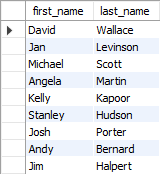
\includegraphics[width=0.4\textwidth]{./Figs/2020-12-24-20-37-08.png}
        % 	\caption{}
        \end{figure}
\end{itemize}
